\chapter{आवर्त सारणी: पहली झलक}\label{ch:g9:periodic-table-first-look}

लगभग हर रसायन विज्ञान कक्षा की दीवार पर एक ही चार्ट टँगा होता है: 118 खाने,
हर एक में एक प्रतीक और एक संख्या, पंक्तियों और स्तंभों में एक अजीब आकृति में
सजे हुए --- दोनों किनारों पर ऊँची मीनारें, बीच में एक गड्ढा, नीचे दो अलग
पंक्तियाँ। जब इसे पहली बार, 1869 में, बनाया गया था, तब इसमें लगभग साठ खाने थे
और कई ख़ाली थे। इसके रचयिता ने उन तत्वों का वर्णन करने का साहस किया जो एक
दिन ख़ाली जगहें भरने वाले थे --- और वे
सही निकले।

\begin{recall}
\omterm{def:g9:inside-the-atom:element}{रासायनिक तत्व} एक ही \omterm{def:g9:inside-the-atom:atomic-number}{परमाणु क्रमांक} $Z$ वाले \omterm{def:g7:atoms-and-molecules:atom}{परमाणुओं} का समुच्चय है, जो
\omterm{def:g9:inside-the-atom:nucleus}{नाभिक} में \omterm{def:g9:inside-the-atom:proton}{प्रोटॉनों} की संख्या है (\cref{ch:g9:inside-the-atom})।
हर तत्व का एक प्रतीक होता है: एक बड़ा अक्षर, जिसके बाद कभी-कभी एक छोटा
अक्षर आता है (\cref{ch:g7:atoms-and-molecules})। लोहा, ज़िंक और ऐलुमिनियम
जैसी \omterm{def:g9:periodic-table-first-look:metal}{धातुएँ} धनात्मक \omterm{def:g9:ions:ion}{आयन} देती हैं (\cref{ch:g9:ions})।
\end{recall}

\section{तत्वों की एक सारणी}

\begin{definition}[आवर्त सारणी]\label{def:g9:periodic-table-first-look:periodic-table}
\emph{आवर्त सारणी}\index{आवर्त सारणी} सभी \omterm{def:g9:inside-the-atom:element}{रासायनिक तत्वों} को बढ़ते
\omterm{def:g9:inside-the-atom:atomic-number}{परमाणु क्रमांक} के क्रम में, $Z = 1$ से $Z = 118$ तक, सूचीबद्ध करती है,
और उन्हें पंक्तियों में ऐसे सजाती है कि मिलते-जुलते गुणों वाले तत्व एक ही
स्तंभ में आएँ।
\end{definition}

\begin{definition}[आवर्त और समूह]\label{def:g9:periodic-table-first-look:period}
\omterm{def:g9:periodic-table-first-look:periodic-table}{आवर्त सारणी} की एक पंक्ति \emph{आवर्त}\index{आवर्त} है; ऐसी सात
हैं। एक स्तंभ \emph{समूह}\index{समूह} है; ऐसे अठारह हैं, जिन्हें बाएँ से
दाएँ 1 से 18 तक क्रमांक दिए गए हैं। सारणी के नीचे छपी दो पंक्तियाँ आवर्त 6
और 7 की हैं; उन्हें केवल सारणी को सँकरा रखने के लिए
अलग रखा गया है।
\end{definition}

\begin{omfigure}
\omperiodictable[colour=metals, legend=true, cell=0.86cm]

{\small \omterm{def:g9:periodic-table-first-look:periodic-table}{आवर्त सारणी}। हर खाने में \omterm{def:g9:inside-the-atom:atomic-number}{परमाणु क्रमांक} और प्रतीक है।
रंग: \omterm{def:g9:periodic-table-first-look:metal}{धातुएँ}, उपधातुएँ (\omterm{def:g9:periodic-table-first-look:metal}{धातुओं} और \omterm{def:g9:periodic-table-first-look:metal}{अधातुओं} के बीच के तत्व) और
\omterm{def:g9:periodic-table-first-look:metal}{अधातुएँ}, सामान्य वर्गीकरण के अनुसार।}
\end{omfigure}

\begin{method}[आवर्त सारणी पढ़ना]\label{met:g9:periodic-table-first-look:read}
किसी तत्व का स्थान जानने के लिए:
\begin{enumerate}
  \item उसके प्रतीक या उसके \omterm{def:g9:inside-the-atom:atomic-number}{परमाणु क्रमांक} से उसका खाना ढूँढो;
  \item उसकी पंक्ति उसका \omterm{def:g9:periodic-table-first-look:period}{आवर्त} बताती है, उसका स्तंभ उसका समूह;
  \item उसका रंग बताता है कि वह \omterm{def:g9:periodic-table-first-look:metal}{धातु} है या \omterm{def:g9:periodic-table-first-look:metal}{अधातु}।
\end{enumerate}
सोडियम, \ce{Na}, $Z = 11$: \omterm{def:g9:periodic-table-first-look:period}{आवर्त} 3, \omterm{def:g9:periodic-table-first-look:period}{समूह} 1, एक \omterm{def:g9:periodic-table-first-look:metal}{धातु}। क्लोरीन,
\ce{Cl}, $Z = 17$: \omterm{def:g9:periodic-table-first-look:period}{आवर्त} 3, \omterm{def:g9:periodic-table-first-look:period}{समूह} 17, एक \omterm{def:g9:periodic-table-first-look:metal}{अधातु}।
\end{method}

\section{धातुएँ और अधातुएँ}

\begin{definition}[धातु और अधातु]\label{def:g9:periodic-table-first-look:metal}
\emph{धातु}\index{धातु} वह तत्व है जो \omterm{def:g6:pure-substances-and-mixtures:pure-substance}{शुद्ध पदार्थ} के रूप में ताज़ा काटने पर
चमकीला होता है, विद्युत और ऊष्मा का अच्छा चालन करता है, मोड़ा या पीटकर आकार
दिया जा सकता है, और धनात्मक \omterm{def:g9:ions:ion}{आयन} बनाता है।
\emph{अधातु}\index{अधातु} में ये गुण नहीं होते: कई गैसें हैं
(ऑक्सीजन, नाइट्रोजन, क्लोरीन), ठोस अधातुएँ धुँधली और भंगुर होती हैं
(सल्फ़र, कोयले के रूप में कार्बन), और वे ऋणात्मक \omterm{def:g9:ions:ion}{आयन} बनाने या \omterm{def:g7:atoms-and-molecules:molecule}{अणुओं} में
\omterm{def:g9:inside-the-atom:nucleus}{इलेक्ट्रॉन} साझा करने की प्रवृत्ति रखती हैं।
\end{definition}

\begin{proposition}[वे कहाँ स्थित हैं]\label{prop:g9:periodic-table-first-look:where}
लगभग हर पाँच में से चार तत्व \omterm{def:g9:periodic-table-first-look:metal}{धातुएँ} हैं; वे सारणी के बाएँ भाग और बीच को भरती
हैं। \omterm{def:g9:periodic-table-first-look:metal}{अधातुएँ} ऊपर दाईं ओर हैं, और हाइड्रोजन अकेली ऊपर बाईं ओर। उनके बीच की
सीमा पर कुछ तत्व --- बोरॉन, सिलिकॉन, जर्मेनियम, आर्सेनिक, ऐंटिमनी, टेल्यूरियम ---
बीच के गुण रखते हैं: ये उपधातुएँ हैं।
\end{proposition}

\section{एक जैसा व्यवहार करने वाले स्तंभ}

\begin{proposition}[एक समूह के तत्व एक जैसा व्यवहार करते हैं]\label{prop:g9:periodic-table-first-look:alike}
एक समूह के तत्व मिलते-जुलते ढंग से अभिक्रिया करते हैं और मिलते-जुलते यौगिक बनाते
हैं। \omterm{def:g9:periodic-table-first-look:period}{समूह} 1 के ऊपर के लिथियम, सोडियम और पोटैशियम नरम \omterm{def:g9:periodic-table-first-look:metal}{धातुएँ} हैं जो पानी के साथ
अभिक्रिया करके हाइड्रोजन देती हैं; समूह में नीचे जाने पर अभिक्रिया अधिक
तीव्र होती है। \omterm{def:g9:periodic-table-first-look:period}{समूह} 17 के फ़्लुओरीन, क्लोरीन, ब्रोमीन और आयोडीन रंगीन \omterm{def:g9:periodic-table-first-look:metal}{अधातुएँ}
हैं जो \omterm{def:g9:periodic-table-first-look:metal}{धातुओं} के साथ अभिक्रिया करके लवण बनाती हैं। हीलियम, नियॉन, आर्गन और \omterm{def:g9:periodic-table-first-look:period}{समूह}
18 के दूसरे तत्व लगभग किसी से अभिक्रिया नहीं करते।
\end{proposition}

\begin{inthelab}[पानी में लिथियम, सोडियम और पोटैशियम]
एक सुरक्षा पर्दे के पीछे शिक्षक चावल के दाने जितना लिथियम का एक टुकड़ा पानी से
भरे बड़े कटोरे में डालते हैं: उसमें हल्की सनसनाहट होती है। उतना ही बड़ा सोडियम का
टुकड़ा सतह पर तेज़ी से घूमता है और पिघलकर चाँदी जैसी गोली बन जाता है। पोटैशियम
तुरंत बैंगनी-गुलाबी लौ के साथ भभक उठता है। तीनों हाइड्रोजन देते हैं और एक
\omterm{def:g9:acids-bases-ph:acidic}{क्षारकीय विलयन} छोड़ते हैं।
\end{inthelab}

\begin{safety}{\ghs[0.82cm]{GHS02}\ghs[0.82cm]{GHS05}}
% ledger: ghs:Na
सोडियम: पानी के संपर्क में यह ज्वलनशील गैसें छोड़ता है जो सुलग सकती हैं
(GHS02); यह गंभीर जलन करता है (GHS05)। इसे तेल में रखा जाता है और केवल
शिक्षक ही चिमटे से, बहुत छोटे टुकड़ों में, इसे सँभालते हैं।
\end{safety}

\section{मेंडेलीव का विचार}

\begin{history}[मेंडेलीव की ख़ाली जगहें, 1869--1886]
1869 में दिमित्री मेंडेलीव ने उस समय ज्ञात तत्वों को बढ़ते \omterm{def:g7:atoms-and-molecules:atom}{परमाणु} भार --- उनके
\omterm{def:g7:atoms-and-molecules:atom}{परमाणुओं} का द्रव्यमान, हाइड्रोजन की तुलना में --- के क्रम में सजाया और मिलते-जुलते
गुणों वाले तत्वों को अगल-बगल रखा। जहाँ पैटर्न की माँग थी, वहाँ उन्होंने उन
तत्वों के लिए ख़ाली जगहें छोड़ीं जिन्हें अभी तक किसी ने नहीं खोजा था, और 1871
में उनके गुणों का वर्णन किया: सिलिकॉन के नीचे एक ``एका-सिलिकॉन'', जिसका \omterm{def:g7:atoms-and-molecules:atom}{परमाणु}
भार लगभग 72 होगा। 1886 में रसायनज्ञ क्लेमेंस विंकलर ने चाँदी के एक \omterm{def:g5:raw-materials-and-recycling:raw-material}{अयस्क} में
जर्मेनियम खोजा, उसका \omterm{def:g7:atoms-and-molecules:atom}{परमाणु} भार 72.3 मापा और पाया कि वही लुप्त तत्व है।
गैलियम (1875) और स्कैंडियम (1879) ने भी मेंडेलीव की छोड़ी ख़ाली जगहें भरीं।
\end{history}

\begin{omfigure}
\begin{minipage}[b]{0.32\linewidth}\centering
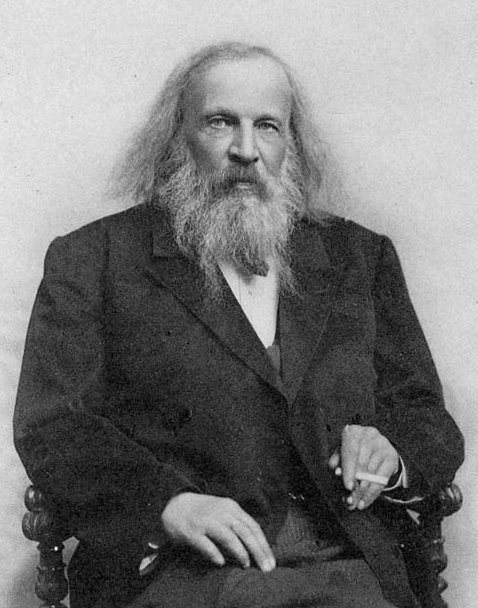
\includegraphics[width=\linewidth]{images/book1/mendeleev.jpg}

{\small दिमित्री मेंडेलीव (1834--1907)।}
\end{minipage}\hfill
\begin{minipage}[b]{0.6\linewidth}\centering
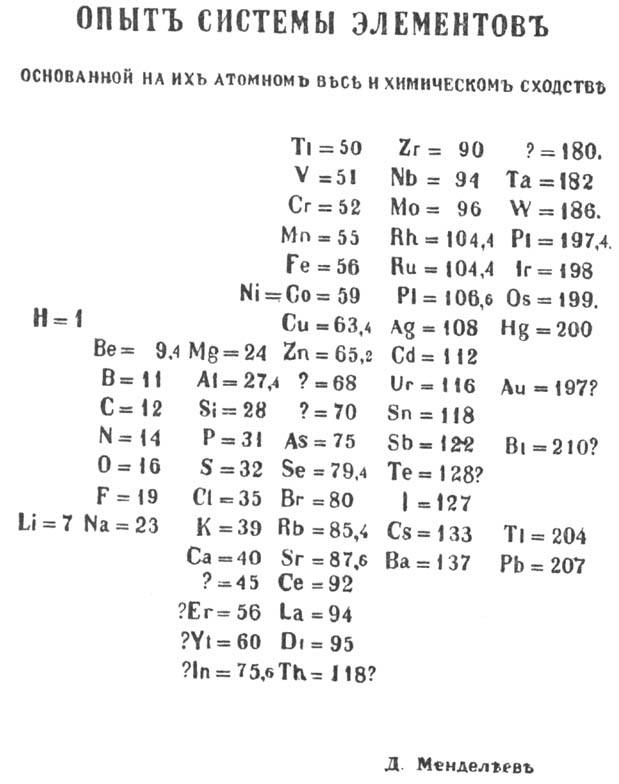
\includegraphics[width=0.85\linewidth]{images/book1/mendeleev-1869.jpg}

{\small 1869 की मेंडेलीव की सारणी, रूसी में। Si $= 28$ और
Al $= 27.4$ के बगल में ख़ाली जगहें ``? $= 70$'' और ``? $= 68$'' जर्मेनियम
और गैलियम की प्रतीक्षा कर रही हैं।}
\end{minipage}
\end{omfigure}

\begin{remark}[परमाणु क्रमांक के अनुसार क्रम]\label{rem:g9:periodic-table-first-look:order}
मेंडेलीव ने तत्वों को \omterm{def:g7:atoms-and-molecules:atom}{परमाणु} भार के अनुसार क्रम दिया, और परिवारों को साथ रखने के
लिए उन्हें टेल्यूरियम और आयोडीन जैसे कुछ जोड़ों की अदला-बदली करनी पड़ी। आज सारणी
\omterm{def:g9:inside-the-atom:atomic-number}{परमाणु क्रमांक} के अनुसार क्रमबद्ध है, जिसकी खोज बाद में हुई, और अदला-बदली की
अब ज़रूरत नहीं।
\end{remark}

\section{अभ्यास}

\begin{exercise}[$\star$]\label{exo:g9:periodic-table-first-look:1}
\omterm{def:g9:periodic-table-first-look:periodic-table}{आवर्त सारणी} में तत्व किस क्रम में रखे जाते हैं?
\end{exercise}

\begin{exercise}[$\star$]\label{exo:g9:periodic-table-first-look:2}
इनके \omterm{def:g9:periodic-table-first-look:period}{आवर्त} और समूह बताओ: कार्बन ($Z = 6$), मैग्नीशियम ($Z = 12$),
आर्गन ($Z = 18$)।
\end{exercise}

\begin{exercise}[$\star$]\label{exo:g9:periodic-table-first-look:3}
\omterm{def:g9:periodic-table-first-look:metal}{धातु} या \omterm{def:g9:periodic-table-first-look:metal}{अधातु}: लोहा, सल्फ़र, ताँबा, ऑक्सीजन, ऐलुमिनियम, क्लोरीन?
\end{exercise}

\begin{exercise}[$\star$]\label{exo:g9:periodic-table-first-look:4}
सारणी में सोडियम के ठीक नीचे कौन-सा तत्व है? क्लोरीन के ठीक नीचे?
\end{exercise}

\begin{exercise}[$\star\star$]\label{exo:g9:periodic-table-first-look:5}
सारणी की मदद से \omterm{def:g9:periodic-table-first-look:period}{आवर्त} 4 और \omterm{def:g9:periodic-table-first-look:period}{समूह} 2 के तत्व का नाम बताओ, और \omterm{def:g9:periodic-table-first-look:period}{आवर्त} 2 और
\omterm{def:g9:periodic-table-first-look:period}{समूह} 15 के तत्व का भी।
\end{exercise}

\begin{exercise}[$\star\star$]\label{exo:g9:periodic-table-first-look:6}
यह उम्मीद क्यों की जा सकती है कि पोटैशियम, सोडियम की तरह, पानी के साथ अभिक्रिया करेगा?
\end{exercise}

\begin{exercise}[$\star\star$]\label{exo:g9:periodic-table-first-look:7}
एक चमकीला तत्व विद्युत का चालन करता है और \omterm{def:g9:ions:ion}{आयन} \ce{X^{2+}} बनाता है। वह
\omterm{def:g9:periodic-table-first-look:metal}{धातु} है या \omterm{def:g9:periodic-table-first-look:metal}{अधातु}? समझाओ।
\end{exercise}

\begin{exercise}[$\star\star$]\label{exo:g9:periodic-table-first-look:8}
मेंडेलीव ने अपनी सारणी में ख़ाली जगहें क्यों छोड़ीं? यह उनकी सारणी की कमज़ोरी के
बजाय ताक़त क्यों थी?
\end{exercise}

\begin{exercise}[$\star\star$]\label{exo:g9:periodic-table-first-look:9}
1869 की मेंडेलीव की सारणी देखो। उन्होंने कार्बन और ऑक्सीजन के लिए कौन-से \omterm{def:g7:atoms-and-molecules:atom}{परमाणु}
भार दिए? प्रश्नचिह्न से चिह्नित कौन-सी दो ख़ाली जगहें ऐलुमिनियम और सिलिकॉन के
बगल में दिखती हैं?
\end{exercise}

\begin{exercise}[$\star\star$]\label{exo:g9:periodic-table-first-look:10}
\omterm{def:g9:periodic-table-first-look:period}{आवर्त} 2 में कितने तत्व हैं? \omterm{def:g9:periodic-table-first-look:period}{आवर्त} 4 में?
\end{exercise}

\begin{exercise}[$\star\star\star$]\label{exo:g9:periodic-table-first-look:11}
हीलियम, नियॉन और आर्गन लगभग किसी से अभिक्रिया नहीं करते। वे किस समूह में
हैं? इस गुण को देखते हुए उनका उपयोग किस काम में हो सकता है?
\end{exercise}

\begin{exercise}[$\star\star\star$]\label{exo:g9:periodic-table-first-look:12}
ऐलुमिनियम के नीचे का गैलियम 1875 में खोजा गया। मेंडेलीव ने उसके लिए अपने पड़ोसियों
ऐलुमिनियम (27.0) और इंडियम (114.8) के औसत के क़रीब \omterm{def:g7:atoms-and-molecules:atom}{परमाणु} भार की भविष्यवाणी
की थी। वह औसत निकालो। (गैलियम: 69.7।)
\end{exercise}

\section{समस्या: मेंडेलीव की ख़ाली जगह}

\begin{problem}[{सप्ताहांत समस्या --- किसी लुप्त तत्व के परमाणु भार की उसके
चार पड़ोसियों से भविष्यवाणी}]
\label{pb:g9:periodic-table-first-look:1}
% ledger: aw:Si, aw:Sn, aw:Ga, aw:As, aw:Ge, mend:eka-si-aw, ge:winkler-aw
1871 में मेंडेलीव ने एका-सिलिकॉन के गुणों की भविष्यवाणी की, जो सिलिकॉन के नीचे
का लुप्त तत्व था। उनका एक विचार यह था कि किसी तत्व के गुण उसके ऊपर और नीचे,
बाएँ और दाएँ के पड़ोसियों के गुणों के बीच होते हैं। ख़ाली जगह के चार पड़ोसियों के
आज के \omterm{def:g7:atoms-and-molecules:atom}{परमाणु} भार ये हैं:
सिलिकॉन 28.1 (ऊपर), टिन 118.7 (नीचे), गैलियम 69.7 (बाएँ), आर्सेनिक
74.9 (दाएँ)।

\medskip
\noindent\textbf{भाग I --- ख़ाली जगह।}
\begin{enumerate}
  \item इस अध्याय की \omterm{def:g9:periodic-table-first-look:periodic-table}{आवर्त सारणी} की मदद से जर्मेनियम का, जो ख़ाली जगह भरने
        वाला तत्व है, \omterm{def:g9:inside-the-atom:atomic-number}{परमाणु क्रमांक}, \omterm{def:g9:periodic-table-first-look:period}{आवर्त} और समूह
        पता करो।
  \item उसके ऊपर कौन-सा तत्व है, नीचे कौन-सा, बाईं ओर कौन-सा, दाईं ओर
        कौन-सा?
  \item जर्मेनियम \omterm{def:g9:periodic-table-first-look:metal}{धातु} है, \omterm{def:g9:periodic-table-first-look:metal}{अधातु} या उपधातु?
  \item मेंडेलीव को यह उम्मीद क्यों थी कि लुप्त तत्व सिलिकॉन से मिलता-जुलता
        होगा?
\end{enumerate}

\medskip
\noindent\textbf{भाग II --- औसत।}
\begin{enumerate}[resume]
  \item ख़ाली जगह के ऊपर और नीचे के तत्वों के \omterm{def:g7:atoms-and-molecules:atom}{परमाणु} भारों का औसत
        निकालो।
  \item बाएँ और दाएँ के तत्वों के \omterm{def:g7:atoms-and-molecules:atom}{परमाणु} भारों का औसत
        निकालो।
  \item दोनों में से कौन-सा औसत जर्मेनियम के वास्तविक \omterm{def:g7:atoms-and-molecules:atom}{परमाणु} भार, 72.6, के अधिक
        क़रीब है? ऐसा क्यों हो सकता है?
  \item अपनी 1869 की सारणी में मेंडेलीव ने इस ख़ाली जगह के लिए ``? $= 70$''
        लिखा था। वे कितना चूके?
\end{enumerate}

\medskip
\noindent\textbf{भाग III --- भविष्यवाणी।}
\begin{enumerate}[resume]
  \item चारों पड़ोसियों का औसत एक दशमलव स्थान तक
        निकालो।
  \item 1871 में मेंडेलीव ने 72 की भविष्यवाणी की; 1886 में विंकलर ने 72.3 मापा।
        अपने औसत से तुलना करो।
  \item जर्मेनियम की खोज ने बहुत-से रसायनज्ञों को क्यों विश्वास दिला दिया कि
        मेंडेलीव की सारणी सही थी?
  \item अपनी भविष्यवाणी बताओ: चार पड़ोसियों के औसत से एका-सिलिकॉन का
        \omterm{def:g7:atoms-and-molecules:atom}{परमाणु} भार।
\end{enumerate}
\end{problem}
